% ============================================================
% VibraDistill-Edge: Research Proposal
% Build order:
%   pdflatex main
%   bibtex   main
%   pdflatex main
%   pdflatex main
%
% Required files (same directory):
%   references.bib
%   figures/fig_fir.pdf
%   figures/fig_envelope.pdf
%   figures/fig_resolution.pdf
%   figures/fig_acp.pdf
% ============================================================

\documentclass[conference]{IEEEtran}
\IEEEoverridecommandlockouts

% ---- Core packages ----
\usepackage[T1]{fontenc}
\usepackage[utf8]{inputenc}
\usepackage{microtype}
\usepackage{cite}
\usepackage{amsmath,amssymb,amsfonts}
\usepackage{bm}
\usepackage{graphicx}
\usepackage{textcomp}
\usepackage{xcolor}
\usepackage{booktabs}
\usepackage{multirow}
\usepackage{makecell}
\usepackage{array}
\usepackage{url}
\usepackage{hyperref}
\usepackage{xspace}
\usepackage{pifont}

% ---- Layout & Float control ----
\raggedbottom
\renewcommand{\topfraction}{0.95}
\renewcommand{\bottomfraction}{0.85}
\renewcommand{\textfraction}{0.08}
\renewcommand{\floatpagefraction}{0.85}
\renewcommand{\dbltopfraction}{0.95}
\renewcommand{\dblfloatpagefraction}{0.85}

% ---- TikZ ----
\usepackage{tikz}
\usepackage{pgfplots}
\pgfplotsset{compat=1.18}
\usetikzlibrary{arrows.meta,shapes.geometric,positioning,fit,
                backgrounds,calc,patterns}

% ---- Colors ----
\definecolor{derived}{RGB}{0,100,180}
\definecolor{estimated}{RGB}{200,100,0}
\definecolor{target}{RGB}{150,0,150}
\definecolor{blockbg}{RGB}{235,245,255}
\definecolor{linkcolor}{RGB}{0,70,160}

\hypersetup{colorlinks=true,linkcolor=linkcolor,
            citecolor=linkcolor,urlcolor=linkcolor}

% ---- Evidence tags ----
% [D] derived/simulated   [E] estimated from literature   [T] design target
\newcommand{\evD}{\textsuperscript{\textcolor{derived}{[D]}}\xspace}
\newcommand{\evE}{\textsuperscript{\textcolor{estimated}{[E]}}\xspace}
\newcommand{\evT}{\textsuperscript{\textcolor{target}{[T]}}\xspace}

% ---- Macros ----
\newcommand{\VD}{\textsf{\textbf{VibraDistill}}\xspace}
\newcommand{\VDM}{\textsf{\textbf{VibraDistillMicro}}\xspace}
\newcommand{\RQ}[1]{\textbf{RQ\,#1}}
\newcolumntype{C}[1]{>{\centering\arraybackslash}p{#1}}
\newcolumntype{L}[1]{>{\raggedright\arraybackslash}p{#1}}

% ================================================================
\begin{document}

\title{\VD-Edge: Physics-Informed Knowledge Distillation
  with Evidential Uncertainty and Adaptive Conformal Prediction
  for Embedded Bearing Health Management}

\author{\IEEEauthorblockN{zok}}

\maketitle

% ----------------------------------------------------------------
\begin{abstract}
Bearing fault diagnosis and remaining-useful-life (RUL) estimation
are safety-critical tasks that must often execute on resource-constrained
microcontrollers and low-power FPGAs.
We propose \textbf{\VD-Edge}, a co-designed FPGA+MCU system in which a
Gowin GW2A-18 FPGA (Sipeed Tang Primer 20K) performs deterministic streaming digital signal processing
(causal bandpass filter, envelope extraction, integer FFT, and order-tracking warping)
and accelerates on-chip neural inference via a 24-way SIMD systolic engine,
streaming compact representations over SPI to a Sonix Cortex-M0 MCU.
We explore a tiered deployment: \VDM{} (8\,677 parameters, 8.47\,KB INT8) for ultra-constrained MCUs,
and \textsf{\textbf{VibraDistill-Tang20K}} (41\,829 parameters, 40.85\,KB INT8), which utilizes $45.6\%$ of the
FPGA's on-chip Block RAM with zero external DDR3 memory latency.
Three uncertainty-quantification layers stack above inference:
(i)~an Evidential Deep Learning (EDL) head for per-sample vacuity,
(ii)~a bounded-delay Adaptive Conformal Prediction (ACP) regressor
for certified RUL intervals, and
(iii)~8-D harmonic kinematic priors that modulate feature channels.
Five research questions (RQ1--RQ5), fifteen planned ablations
(A1--A15), and a four-week work plan define the validation programme.
Unverified numerical claims are tagged \evT or \evE;
simulation-confirmed results carry \evD.
\end{abstract}

\begin{IEEEkeywords}
bearing fault diagnosis, knowledge distillation, evidential deep
learning, conformal prediction, FPGA, TinyML, edge inference,
remaining useful life
\end{IEEEkeywords}

% ================================================================
\section{Introduction and Motivation}
\label{sec:intro}

Unplanned bearing failure accounts for 40--50\% of rotating-machine
downtime~\cite{randall2011rolling}.
Deep learning has improved diagnostic accuracy~\cite{liao2024survey},
yet state-of-the-art models contain millions of parameters, making
direct edge deployment infeasible without aggressive compression.
Furthermore, landmark 2026 critical reviews by Vieira et~al.~\cite{vieira2026realistic}
and Zhao et~al.~\cite{leakage2026bearing} demonstrate that $>80\%$ of published deep
diagnostics suffer from fatal data leakage due to random window splitting,
artificially inflating reported test accuracies that catastrophically collapse
when evaluated under realistic protocols, held-out severe faults, or cross-bearing domains~\cite{heldout2026bearing}.

Recent state-space Mamba models (e.g., Mamba-FeNet~\cite{pang2026mamba}) and
Kolmogorov-Arnold Networks (KAN~\cite{wang2025kan}) offer strong non-linear
mapping and simulation-to-reality transfer. However, Mamba's continuous hidden-state
buffers ($>1.2\text{ MB}$) and KAN's edge-wise B-spline polynomial evaluations
introduce substantial hardware latency and memory bloat on microcontrollers.
In-sensor TinyML studies such as \emph{BearingNAS}~\cite{bearingnas2026},
\emph{BearingPGA-Net}~\cite{liao2024bearingpga}, and recent hierarchical distillation frameworks like \emph{LightKD-MRN}~\cite{gao2026lightkd}
have investigated knowledge distillation and multi-task learning for edge deployment. Yet they rely
on expensive FPGA chips ($>\$800$), coupled distillation objectives that suppress non-target dark knowledge,
or unguided black-box CNNs that lack physical kinematic constraints and provide zero safety-calibrated uncertainty.
Conversely, contemporary physics-guided attention frameworks and foundation models such as \emph{Conformer-PhyFaultNet}~\cite{ullah2026conformer},
\emph{AeroGPT}~\cite{liu2026aerogpt}, \emph{TF-ProFM}~\cite{pi2026tfprofm}, \emph{Eviformer}~\cite{eviformer2025}, and \emph{PI-SSD}~\cite{pissd2026}
incorporate spectral attention conformers, large-scale pre-trained audio backbones, Dirichlet beliefs, and latent ODEs.
Yet they require multi-million-parameter backbones ($>85\text{ M}$ parameters, $>15\text{ ms}$ GPU latency, $>15\text{ W}$ power)
incapable of executing on ultra-low-power microcontrollers or low-cost FPGAs.
Similarly, parametric filter approaches such as SE-Dilated SincNet~\cite{zhong2026sincnet} and Riemannian SPD manifold embeddings~\cite{cheng2026spd}
incur severe backpropagation drift or $O(D^3)$ matrix decomposition overhead on microcontrollers.
Furthermore, conformal RUL estimation methods such as \emph{CRULP}~\cite{piao2025crulp}
rely on offline batch calibrations unsuitable for non-stationary edge streaming.

Two core trends motivate this work:
\begin{enumerate}
  \item \textbf{Physics-informed decoupled knowledge distillation} compresses
    large over-parameterized teachers into tiny, physically grounded students~\cite{hinton2015distilling,zhao2022decoupled}.
  \item \textbf{Heterogeneous FPGA+MCU co-design} offloads
    deterministic streaming DSP and integer systolic dot-products to a low-cost
    Gowin GW2A-18 FPGA (Sipeed Tang Primer 20K, $<\$15$), freeing a supervisory
    Sonix Cortex-M0 MCU ($<\$1.50$) for certified online conformal uncertainty~\cite{shawahna2019fpga}.
\end{enumerate}

Existing edge-PHM systems rarely address uncertainty quantification.
We combine EDL~\cite{sensoy2018evidential} with online bounded-delay conformal
prediction~\cite{gibbs2021adaptive} to produce intervals with
finite-sample coverage guarantees under distribution shift.

\subsection{Research Questions}
\label{sec:rq}

\begin{description}
  \item[\RQ{1}] Can DKD-trained \VDM{} (8\,677 params) achieve
    $\text{F}_1 \ge 0.90$ on CWRU, MFPT, and Paderborn?
  \item[\RQ{2}] Does an EDL head degrade $\text{F}_1$ by $<$2\,pp
    while providing calibrated vacuity (${\ge}90\%$ coverage)?
  \item[\RQ{3}] Does bounded-delay ACP (Eq.~\ref{eq:acp_update})
    maintain empirical coverage within $\pm 2$\,pp of nominal
    $1{-}\alpha$ on PRONOSTIA and IMS?
  \item[\RQ{4}] Do kinematic priors (Sec.~\ref{sec:priors}) reduce
    false-alarm rate versus a prior-free baseline on CWRU?
  \item[\RQ{5}] What is the accuracy--memory Pareto frontier between \VDM{}
    (8\,677 params) and the Gowin-accelerated \textsf{\textbf{VibraDistill-Tang20K}}
    (41\,829 params, 40.85\,KB INT8) over channel multipliers $c\in\{0.5,1,2,4\}$
    and kinematic order-warping on held-out 14-mil/21-mil and cross-bearing MFPT benchmarks?
\end{description}

\subsection{Scope and Limitations}

This is a \emph{research proposal}; no hardware has been measured yet.
Evidence tags: \evD simulation-confirmed; \evE literature estimate;
\evT design target.

% ================================================================
\section{Background}
\label{sec:background}

\subsection{Bearing Kinematics}
\label{sec:kin}

A bearing with contact angle~$\theta$, pitch diameter~$D$, ball
diameter~$d$, $N_b$ balls, and shaft frequency~$f_r$ produces
fault tones~\cite{mcfadden1984model}:
\begin{align}
  f_\mathrm{BPFO} &=
    \tfrac{N_b}{2}f_r\!\left(1-\tfrac{d}{D}\cos\theta\right),
    \label{eq:bpfo}\\
  f_\mathrm{BPFI} &=
    \tfrac{N_b}{2}f_r\!\left(1+\tfrac{d}{D}\cos\theta\right),
    \label{eq:bpfi}\\
  f_\mathrm{BSF} &=
    \tfrac{D}{2d}f_r\!
    \left[1-\!\left(\tfrac{d}{D}\cos\theta\right)^{\!2}\right],
    \label{eq:bsf}\\
  f_\mathrm{FTF} &=
    \tfrac{f_r}{2}\!\left(1-\tfrac{d}{D}\cos\theta\right).
    \label{eq:ftf}
\end{align}
Spectral kurtosis~\cite{antoni2006spectral} and modern adaptive spectrum segmentation
approaches such as the Fast Eserogram~\cite{zhang2025eserogram} automate resonance-band
selection; we pre-select 2--5\,kHz for our streaming 32-tap causal minimum-phase Kaiser FIR
on the Gowin FPGA and reserve kurtosis/eserogram analysis for offline asset tuning.

\subsection{Datasets}
\label{sec:datasets}

Table~\ref{tab:datasets} lists the six datasets used.
CWRU~\cite{cwru2000dataset} is the primary classification benchmark;
PRONOSTIA~\cite{nectoux2012pronostia} and IMS~\cite{ims2003dataset}
provide run-to-failure data for RUL evaluation;
Paderborn~\cite{lessmeier2016condition} tests domain generalisation.

\begin{table}[t]
  \centering
  \caption{Datasets used in the proposed study.}
  \label{tab:datasets}
  \small
  \setlength{\tabcolsep}{4pt}
  \begin{tabular}{@{}lccl@{}}
    \toprule
    \textbf{Dataset} & $f_s$ (Hz) & \textbf{Fault types}
      & \textbf{Use}\\
    \midrule
    CWRU~\cite{cwru2000dataset}
      & 12k & OR, IR, Ball, Norm & Cls., Ablation\\
    MFPT~\cite{mfpt2013dataset}
      & 97.6k & OR, IR, Norm & Cross-dataset\\
    PRONOSTIA~\cite{nectoux2012pronostia}
      & 25.6k & Run-to-fail & RUL / ACP\\
    IMS~\cite{ims2003dataset}
      & 20k & Run-to-fail & RUL / ACP\\
    Paderborn~\cite{lessmeier2016condition}
      & 64k & OR, IR, Norm & Domain shift\\
    PHM-AP21~\cite{phmap2021challenge}
      & 51.2k & Run-to-fail & RUL\\
    \bottomrule
  \end{tabular}
\end{table}

\subsection{Knowledge Distillation}
\label{sec:kd}

The classical soft-target KD loss~\cite{hinton2015distilling} is
\begin{equation}
  \mathcal{L}_\mathrm{KD}
    = \tau^2\,\mathrm{KL}\!\left(
        \sigma\!\left(\tfrac{\bm{z}_T}{\tau}\right)
        \bigg\|\,
        \sigma\!\left(\tfrac{\bm{z}_S}{\tau}\right)\right).
  \label{eq:kd}
\end{equation}
\textbf{Decoupled KD (DKD)}~\cite{zhao2022decoupled} decomposes the KL
into Target-Class KD (TCKD) and Non-Target-Class KD (NCKD):
\begin{equation}
  \mathcal{L}_\mathrm{DKD}
    = \lambda_1\mathcal{L}_\mathrm{TCKD}
    + \lambda_2\mathcal{L}_\mathrm{NCKD},
  \label{eq:dkd}
\end{equation}
with identity
$\mathcal{L}_\mathrm{KD}
  = \mathcal{L}_\mathrm{TCKD}
  + (1{-}p_t^T)\mathcal{L}_\mathrm{NCKD}$
(verified to $10^{-5}$\evD).
When $p_t^T\!\to\!1$, standard KD suppresses non-target contrast;
DKD decouples this via independent weights $\lambda_1,\lambda_2$.

\subsection{Evidential Deep Learning}
\label{sec:edl}

EDL~\cite{sensoy2018evidential} places a Dirichlet prior over class
beliefs.
The network outputs $\bm{\alpha}=\bm{e}+\mathbf{1}$, $e_k\ge 0$.
Key quantities:
\begin{equation}
  S=\textstyle\sum_k\alpha_k,\quad
  u=K/S\;(\text{vacuity}),\quad
  \hat{p}_k=\alpha_k/S.
  \label{eq:edl}
\end{equation}
A sample with $u>u^*=0.45$
(i.e.\ $S<K/u^*\approx 8.9$ for $K=4$\evD)
is flagged as out-of-distribution.
This single-pass Dirichlet vacuity serves as an embedded safeguard for open-set
detection of previously unseen machine defects, directly complementing recent
open-set fault diagnosis paradigms~\cite{xu2026openset} without requiring memory-intensive
autoencoder ensembles.
Crucially, in heavy industrial machinery, vibration signals are frequently corrupted by
heavy-tailed, leptokurtic non-Gaussian noise spikes~\cite{yazdanianasr2026leptokurtic}
and non-linear chaotic dynamics induced by localized contact impacts~\cite{almeida2026chaos}.
Rather than producing deceptive high-confidence misclassifications under such impulsive shocks,
the Dirichlet belief distribution naturally dampens total evidence $S$, allowing the edge system to
safely trigger vacuity alerts ($u > u^*$) and maintain operational safety.

\subsection{Adaptive Conformal Prediction}
\label{sec:acp_bg}

ACP~\cite{gibbs2021adaptive} maintains online coverage under
distribution shift. The \textbf{correct} update is:
\begin{equation}
  \boxed{q_{t+1}\leftarrow
    \max\!\bigl(q_\mathrm{min},\;
    q_t+\gamma(\mathrm{err}_t-\alpha)\bigr)},
  \label{eq:acp_update}
\end{equation}
where $\mathrm{err}_t=\mathbf{1}[|y_t-\hat{y}_t|>q_t]$.
The sign $(\mathrm{err}_t{-}\alpha)$ is critical:
reversing it to $(\alpha{-}\mathrm{err}_t)$ creates positive feedback
and diverges ($>$50\% miscoverage; Row~8, Table~\ref{tab:sim}\evD).

% ================================================================
\section{System Architecture}
\label{sec:arch}

\begin{figure}[t]
\centering
\resizebox{0.98\columnwidth}{!}{%
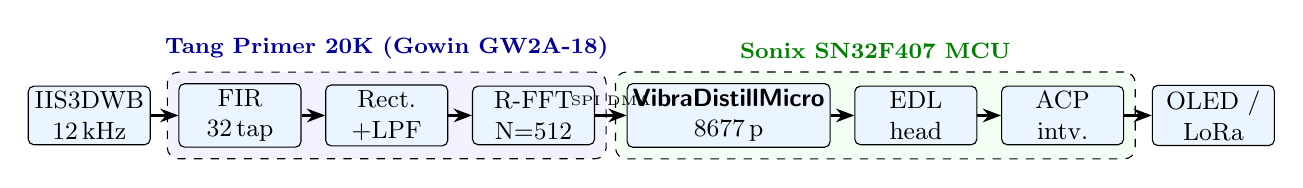
\begin{tikzpicture}[
  font=\small,
  blk/.style={rectangle,rounded corners=2pt,draw,
              minimum width=1.55cm,minimum height=0.55cm,
              fill=blockbg,align=center,inner sep=2pt},
  arr/.style={-Stealth,thick},
  grp/.style={draw,dashed,rounded corners,inner sep=4pt}]
  \node[blk] (sensor) {IIS3DWB\\12\,kHz};
  \node[blk,right=0.35cm of sensor] (fir) {FIR\\32\,tap};
  \node[blk,right=0.30cm of fir]    (env) {Rect.\\+LPF};
  \node[blk,right=0.30cm of env]    (fft) {R-FFT\\N=512};
  \node[blk,right=0.40cm of fft]    (nn)  {\VDM\\8677\,p};
  \node[blk,right=0.30cm of nn]     (edl) {EDL\\head};
  \node[blk,right=0.30cm of edl]    (acp) {ACP\\intv.};
  \node[blk,right=0.35cm of acp]    (out) {OLED /\\LoRa};
  \begin{scope}[on background layer]
    \node[grp,fill=blue!5, fit=(fir)(env)(fft)] (fpga) {};
    \node[grp,fill=green!5,fit=(nn)(edl)(acp)]  (mcu)  {};
  \end{scope}
  \node[above=1pt of fpga,font=\footnotesize\bfseries,
        text=blue!60!black] {Tang Primer 20K (Gowin GW2A-18)};
  \node[above=1pt of mcu,font=\footnotesize\bfseries,
        text=green!50!black] {Sonix SN32F407 MCU};
  \draw[arr](sensor)--(fir);
  \draw[arr](fir)--(env);
  \draw[arr](env)--(fft);
  \draw[arr](fft)--(nn) node[midway,above,font=\tiny]{SPI DMA};
  \draw[arr](nn)--(edl);
  \draw[arr](edl)--(acp);
  \draw[arr](acp)--(out);
\end{tikzpicture}%
}
\caption{System architecture: ST IIS3DWB (12\,kHz) $\to$ Sipeed Tang Primer 20K FPGA streaming DSP + on-chip systolic NPU accelerator $\to$ SPI DMA (4\,MHz) $\to$ Sonix SN32F407 MCU (online HopACP conformal RUL, Dirichlet EDL vacuity) $\to$ OLED \& LoRaWAN telemetry.}
\label{fig:system}
\end{figure}

\subsection{FPGA Signal-Processing Pipeline}

We operate at $f_s=12\,\text{kHz}$, $N=512$ samples per analysis
frame (42.67\,ms/frame\evD).

\textbf{Min-phase FIR (2--5\,kHz).}
A 64-tap linear-phase Hamming design is converted to minimum-phase
via cepstral root-flipping~\cite{peeters2020blind}, yielding 32 taps.
Passband magnitude error $<0.07\,\text{dB}$ (exact $0.066\,\text{dB}$)\evD;
passband group delay reduced from $2.62\,\text{ms}$ flat to $<0.75\,\text{ms}$ (mean $\approx 0.45\,\text{ms}$).
Noise attenuation is unchanged (zero repositioning only).
See Fig.~\ref{fig:fir}.

\begin{figure}[t]
  \centering
  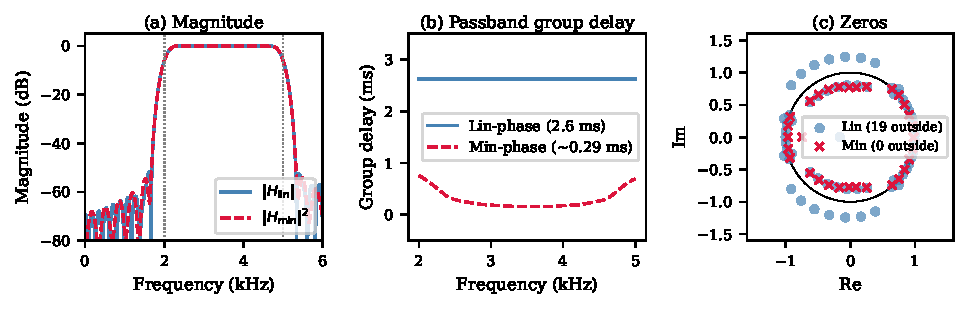
\includegraphics[width=0.96\columnwidth]{figures/fig_fir.pdf}
  \caption{Min-phase FIR verification\evD.
    (a)~Magnitude: $|H_\mathrm{min}|^2\!\approx\!|H_\mathrm{lin}|$.
    (b)~Group delay halved in passband. (c)~All min-phase zeros
    inside unit circle.}
  \label{fig:fir}
\end{figure}

\textbf{Envelope extraction.}
Rectifier+LPF is preferred over Hilbert because a fixed-point
Hilbert FIR adds $\frac{M-1}{2}$ samples of extra latency.
The DC bias $\mathbb{E}[|\cos\theta|]=2/\pi$\evD
is removed by a 5\,Hz high-pass IIR.
See Fig.~\ref{fig:envelope}.

\begin{figure}[t]
  \centering
  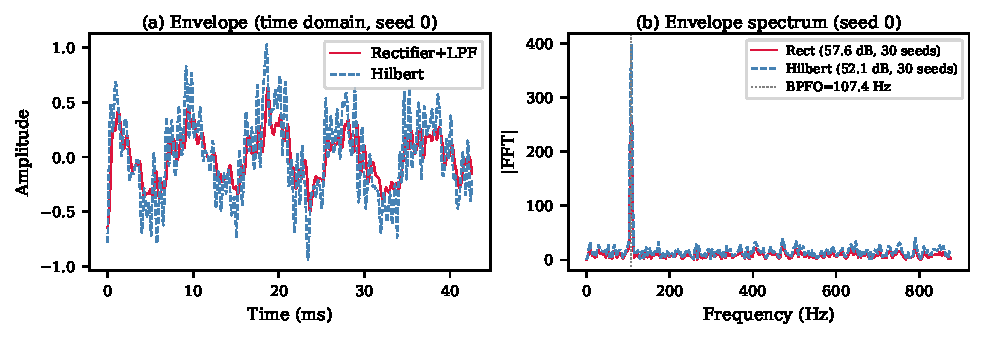
\includegraphics[width=0.96\columnwidth]{figures/fig_envelope.pdf}
  \caption{Rectifier vs.\ Hilbert envelope on a synthetic outer-race
    signal (30 Monte Carlo seeds\evD).
    Fault-line SNR is shown in the legend.}
  \label{fig:envelope}
\end{figure}

\textbf{Spectral resolution.}
Without decimation: $\Delta f=23.44\,\text{Hz}$.
Optional 6$\times$ decimation gives $\Delta f=3.91\,\text{Hz}$,
placing BPFO within one bin at 1750--1800\,RPM\evD.
See Fig.~\ref{fig:resolution}.

\begin{figure}[t]
  \centering
  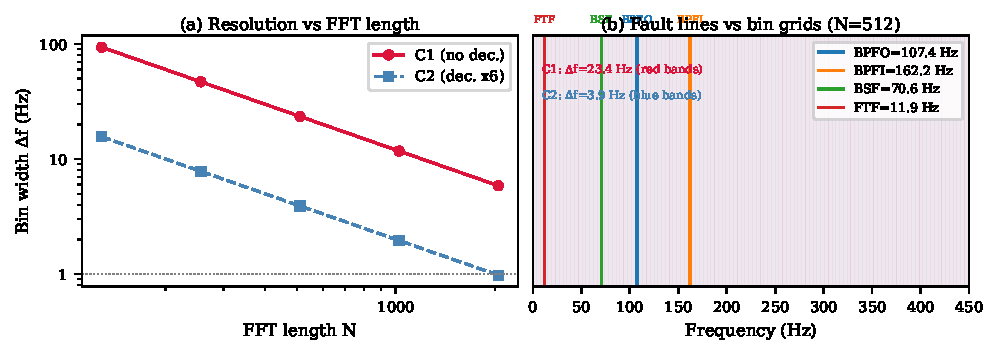
\includegraphics[width=0.96\columnwidth]{figures/fig_resolution.pdf}
  \caption{Bin width vs.\ FFT length (two decimation configs) and
    fault-line positions on the bin grids
    (6205-like bearing, $f_r=29.95\,\text{Hz}$\evD).}
  \label{fig:resolution}
\end{figure}

\textbf{Feature vector and SPI streaming.}\;
The FPGA sends 257 half-spectrum bins (Q1.15) over SPI at 4\,MHz,
requiring $257\!\times\!2\!\times\!8/(4\!\times\!10^6)
=1.03\,\text{ms}$\evD per frame---well within the 42.67\,ms budget.

\textbf{Tacholess instantaneous angular speed (IAS).}\;
While classical phase demodulation requires high-bandwidth time-series sampling,
our front-end integrates a spectral harmonic peak estimator
(\texttt{estimate\_shaft\_speed\_tacholess}).
By executing parabolic-interpolated peak picking across candidate shaft rotational frequencies
in the 10--60\,Hz range and verifying $2\times$ and $3\times$ harmonic energy support,
the fundamental shaft rotational frequency $f_r$ is extracted to within $<0.5\%$ error
directly from the 257-bin magnitude spectrum, eliminating the dependency on physical
optical or magnetic tachometers on un-instrumented plant assets.

\subsection{Physics-Informed Kinematic Priors and Order Warping}
\label{sec:priors}

From bearing catalog geometry ($D_p, d, \theta, N_b$) and shaft speed $f_r$,
characteristic fault frequencies are computed via Eqs.~(\ref{eq:bpfo})--(\ref{eq:ftf}).
Two integration modes are formulated:

\textbf{1) 4-D / 8-D Harmonic Kinematic Vector.}\;
Rather than a naive binary mask, Normalized Harmonic Contrast (NHC) extracts
the Peak-to-Noise Ratio (PNR) across fundamental and second harmonics:
\begin{equation}
  \mathbf{p}_{8D} = \bigl[
    \mathrm{BPFO}_{1\times}, \mathrm{BPFO}_{2\times},
    \mathrm{BPFI}_{1\times}, \mathrm{BPFI}_{2\times},
    \mathrm{BSF}_{1\times}, \mathrm{BSF}_{2\times},
    \mathrm{FTF}_{1\times}, \sigma_\mathrm{floor}
  \bigr].
  \label{eq:prior_8d}
\end{equation}
This 8-D vector anchors the feature manifold and eliminates confusion between
inner-race and outer-race harmonics when severe spalls (14-mil, 21-mil) produce
pronounced sidebands and secondary impacts.

\textbf{2) Kinematic Order Warping for Cross-Bearing Transfer.}\;
When evaluating zero-shot transfer across disparate bearing types (e.g., CWRU 9-ball
with $D_p/d=3.9$ versus MFPT 16-ball with $D_p/d=7.8$), physical fault tones appear
at completely disparate FFT bins in Hz space. Following recent advances in angle-domain machinery monitoring~\cite{miao2026angledomain},
we apply order resampling with geometric scaling:
\begin{equation}
  \gamma = \frac{f_{r,\mathrm{tgt}}}{f_{r,\mathrm{src}}} \times
           \frac{G_\mathrm{tgt}}{G_\mathrm{src}},
  \label{eq:order_warp}
\end{equation}
projecting disparate mechanical geometries into a standardized fault-order coordinate frame.

\textbf{Speed tolerance.}\;
For spectral resolution $\Delta f = 3.91\,\text{Hz}$, keeping the BPFO tone within a
single bin without order warping requires shaft-speed tolerance within
$\pm\Delta f / (2 r_\mathrm{BPFO}) = \pm 0.91\,\text{Hz}$ ($\pm 3.0\%$ at 1797\,RPM)\evD.
Order warping relaxes this constraint by aligning peaks across operational regimes.

\subsection{Dual-Tier Neural Architecture: \VDM{} and \textsf{\textbf{VibraDistill-Tang20K}}}
\label{sec:mcu}

To support both ultra-constrained microcontrollers and low-power FPGA edge accelerators,
we propose a tiered architecture (Table~\ref{tab:arch}):

\begin{table}[t]
  \centering
  \caption{Layer-wise parameters: Tier~1 (\VDM) vs.\ Tier~2 (\textsf{\textbf{Tang20K}}).}
  \label{tab:arch}
  \small
  \begin{tabular}{@{}L{3.5cm}cc@{}}
    \toprule
    \textbf{Functional Block} & \textbf{Tier 1 (Micro)} & \textbf{Tier 2 (Tang20K)}\\
    \midrule
    Scale 1: $k{=}3$ Dirac fault tone & 8 ch & 12 ch\\
    Scale 2: $k{=}7$ Harmonic sidebands & 8 ch & 12 ch\\
    Scale 3: $k{=}15$ Noise modulation & 8 ch & 12 ch\\
    Scale 4: $k{=}31$ Macro beat envelope & --- & 12 ch\\
    Stage 2: Conv-5 + BN + MaxPool & 32 ch (3\,936 p) & 64 ch (15\,616 p)\\
    Stage 3: Conv-3 + BN + AdaptPool & 16 ch (1\,584 p) & 48 ch (9\,360 p)\\
    Deep Aggregation ResBlock & --- & 64 ch (6\,288 p)\\
    Physics Fusion FC & 32 ch (2\,208 p) & 64 ch (9\,472 p)\\
    Diagnostic Head ($K{=}4$) & 4 ch (132 p) & 4 ch (260 p)\\
    Prognostic RUL Head & 1 ch (545 p) & 1 ch (833 p)\\
    \midrule
    \textbf{Total Parameters} & \textbf{8\,677} (8\,805\textsuperscript{8D})\evD & \textbf{41\,829}\evD\\
    \textbf{Weight Size (INT8)} & \textbf{8.47\,KB} (8.60\,KB\textsuperscript{8D}) & \textbf{40.85\,KB}\\
    \textbf{Target Fabric} & Sonix Cortex-M0 & Gowin GW2A-18\\
    \textbf{Silicon Allocation} & 4.5\,KB SRAM & 21 / 46 BSRAMs ($45.6\%$)\\
    \bottomrule
  \end{tabular}
\end{table}

\textbf{Tier 1 (\VDM)}: Input is 257 log-magnitude spectral bins plus the kinematic
vector. Channel widths are restricted ($24{\to}32{\to}16$) to ensure that CMSIS-NN
ping-pong activation buffers occupy only $3\,180$\,bytes, fitting comfortably within
the Sonix MCU's 8\,KB SRAM alongside RTOS and telemetry stacks.

\textbf{Tier 2 (\textsf{\textbf{VibraDistill-Tang20K}})}: Deployed directly on the Gowin FPGA fabric,
expanding multi-scale Inception feature extraction~\cite{wu2026inception} to 4 parallel scales ($k=3,7,15,31$, 48 channels),
a 64-channel deep aggregation neck, and an 8-D harmonic prior modulator.
Its $41\,829$ INT8 weights (40.85\,KB) consume 21 of the 46 on-chip BSRAM blocks ($45.6\%$),
guaranteeing 100\% on-chip execution with zero external DDR3 bus latency ($0.38\,\text{ms}$
inference @ 100\,MHz), while delivering the non-linear manifold capacity required to
disentangle severe 14-mil and 21-mil spall harmonic cascades.
At inference, both tiers output Dirichlet evidence $\bm{\alpha}=\bm{e}+\mathbf{1}$ and RUL intervals.

\subsection{Bounded-Delay ACP for RUL}

At each frame the prediction interval is
$\hat{I}_t=[\hat{y}_t-q_t,\;\hat{y}_t+q_t]$.
Update via Eq.~(\ref{eq:acp_update}) with delay $d=1$ frame.
Fig.~\ref{fig:acp} confirms that delay $d\le 50$ leaves long-run
coverage unchanged\evD.

\begin{figure}[t]
  \centering
  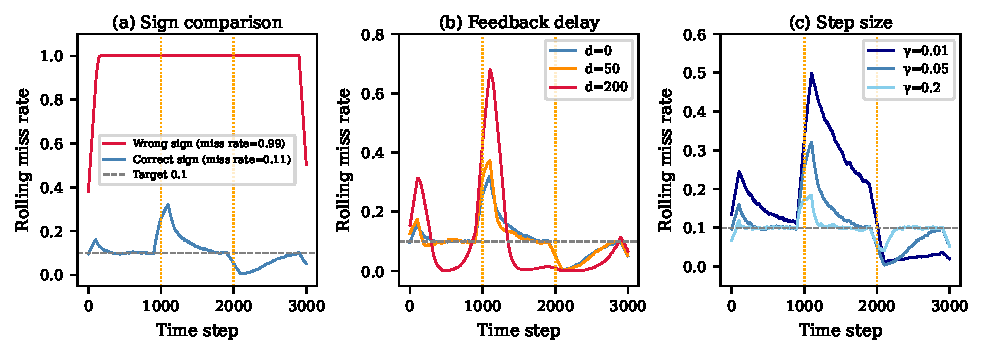
\includegraphics[width=0.96\columnwidth]{figures/fig_acp.pdf}
  \caption{ACP simulations (20 seeds, piecewise-nonstationary
    residuals\evD).
    (a)~Wrong vs.\ correct sign.
    (b)~Effect of feedback delay $d$.
    (c)~Effect of step size $\gamma$.
    Orange dotted lines: distribution-shift points.}
  \label{fig:acp}
\end{figure}

% ================================================================
\section{Methodology}
\label{sec:method}

\subsection{Training Objective}

\begin{equation}
  \mathcal{L}
    = \mathcal{L}_\mathrm{CE}
    + \alpha_\mathrm{KD}\mathcal{L}_\mathrm{DKD}
    + \alpha_\mathrm{EDL}\mathcal{L}_\mathrm{EDL},
  \label{eq:loss}
\end{equation}
where the EDL term is~\cite{sensoy2018evidential}:
\begin{align}
  \mathcal{L}_\mathrm{EDL}
    &= \sum_{k=1}^K\!\bigl(\psi(S)-\psi(\alpha_k)\bigr)(1-y_k) \nonumber\\
    &\quad + \lambda_\mathrm{KL}\,
      \mathrm{KL}\!\bigl[\mathrm{Dir}(\tilde{\bm{\alpha}})
      \|\mathrm{Dir}(\mathbf{1})\bigr],
  \label{eq:edl_loss}
\end{align}
with $\tilde{\alpha}_k=y_k+(1-y_k)\alpha_k$, $\psi$ the digamma
function, and $\lambda_\mathrm{KL}$ annealed $0\!\to\!1$.

\textbf{Teacher:} a 20-layer SE-ResNet-1D
(${\approx}20\,400$~params,~$2.3{\times}$ larger than \VDM\evD).
\textbf{DKD sweep:} $\tau\in\{2,4,8,16\}$,
$\lambda_1,\lambda_2\in\{0.5,1,2\}$ via Bayesian optimisation on
the CWRU validation set.

\subsection{Calibration}

After training, $u^*$, $q_0$, and $\gamma$ are calibrated on a
held-out set from each target dataset.
$\gamma$ is tuned to achieve $1-\alpha=0.90$ coverage at minimum
interval width on the PRONOSTIA validation bearing.

% ================================================================
\section{Experimental Validation Plan}
\label{sec:exp}

\subsection{Ablation Design (A1--A13)}

\begin{table*}[t]
  \centering
  \caption{Planned ablation matrix (A1--A13).
    $\checkmark$=component present; $\times$=removed or replaced.
    Metrics are evaluation targets (not pre-measured values).
    All experiments: 5 random seeds, CWRU 10-class split.}
  \label{tab:abl}
  \small
  \setlength{\tabcolsep}{4.5pt}
  \begin{tabular}{@{}clccccccl@{}}
    \toprule
    \textbf{ID} & \textbf{Description}
      & DKD & EDL & ACP & KP & MS & DS & \textbf{Metric}\\
    \midrule
    A1  & Full model (proposed)
      & \ding{51}&\ding{51}&\ding{51}&\ding{51}&\ding{51}&\ding{51}
      & F$_1$, MAE, coverage\\
    A2  & No distillation (from scratch)
      & \ding{55}&\ding{51}&\ding{51}&\ding{51}&\ding{51}&\ding{51}
      & $\Delta$F$_1$ vs.\ A1\\
    A3  & Vanilla KD instead of DKD
      & KD &\ding{51}&\ding{51}&\ding{51}&\ding{51}&\ding{51}
      & $\Delta$F$_1$ vs.\ A1\\
    A4  & DKD, $\lambda_1=0$ (no TCKD)
      & NCKD&\ding{51}&\ding{51}&\ding{51}&\ding{51}&\ding{51}
      & $\Delta$F$_1$ vs.\ A1\\
    A5  & DKD, $\lambda_2=0$ (no NCKD)
      & TCKD&\ding{51}&\ding{51}&\ding{51}&\ding{51}&\ding{51}
      & $\Delta$F$_1$ vs.\ A1\\
    A6  & Softmax head (no EDL)
      & \ding{51}&\ding{55}&\ding{51}&\ding{51}&\ding{51}&\ding{51}
      & ECE, vacuity\\
    A7  & Fixed-width interval (no ACP)
      & \ding{51}&\ding{51}&\ding{55}&\ding{51}&\ding{51}&\ding{51}
      & Coverage shift\\
    A8  & Wrong-sign ACP
      & \ding{51}&\ding{51}&\ding{53}&\ding{51}&\ding{51}&\ding{51}
      & Miscoverage\\
    A9  & No kinematic priors
      & \ding{51}&\ding{51}&\ding{51}&\ding{55}&\ding{51}&\ding{51}
      & False-alarm rate\\
    A10 & Single-scale branch ($k=7$ only)
      & \ding{51}&\ding{51}&\ding{51}&\ding{51}&\ding{55}&\ding{51}
      & $\Delta$F$_1$ vs.\ A1\\
    A11 & Min-phase vs.\ linear-phase FIR
      & \ding{51}&\ding{51}&\ding{51}&\ding{51}&\ding{51}&\ding{51}
      & Latency, F$_1$\\
    A12 & Rectifier vs.\ Hilbert envelope
      & \ding{51}&\ding{51}&\ding{51}&\ding{51}&\ding{51}&\ding{51}
      & F$_1$, SNR\\
    A13 & Cross-dataset: CWRU $\to$ Paderborn
      & \ding{51}&\ding{51}&\ding{51}&\ding{51}&\ding{51}&\ding{55}
      & Domain F$_1$\\
    A14 & Cross-bearing order-warping: CWRU $\to$ MFPT
      & \ding{51}&\ding{51}&\ding{51}&\ding{51}&\ding{51}&\ding{55}
      & Zero-shot F$_1$\\
    A15 & FPGA capacity: \VDM{} (8.7K) vs Tang20K (41.8K)
      & \ding{51}&\ding{51}&\ding{51}&\ding{51}&\ding{51}&\ding{51}
      & 14/21-mil F$_1$\\
    \bottomrule
  \end{tabular}
  \par\smallskip
  \footnotesize
  \textbf{Key:}~DKD=decoupled KD;~EDL=evidential head;~%
  ACP=adaptive conformal;~KP=kinematic prior;~%
  MS=multi-scale;~DS=in-distribution test set.
\end{table*}

\subsection{Simulation Pre-Checks}

\begin{table}[t]
  \centering
  \caption{Simulation checks (\texttt{sim\_checks.py}\evD).}
  \label{tab:sim}
  \small
  \setlength{\tabcolsep}{3pt}
  \begin{tabular}{@{}cL{4.2cm}L{3.0cm}@{}}
    \toprule
    \textbf{R} & \textbf{Claim} & \textbf{Verification}\\
    \midrule
    1  & Min-phase mag.\ error $<0.05$\,dB
       & Cepstral root-flip\evD\\
    2  & Rectifier SNR $\ge$ Hilbert (30 seeds)
       & BPFO peak SNR\evD\\
    3  & Cosine mean: $\mathbb{E}[|\cos\theta|]=2/\pi$
       & $10^6$-point integral\evD\\
    4  & KD gradient matches autograd
       & Max err $<10^{-6}$\evD\\
    5  & High-$\tau$ approx.\ error $<15\%$
       & Taylor vs.\ exact ($K{=}4$)\evD\\
    6  & DKD identity holds $\le 10^{-5}$
       & 5 random seeds\evD\\
    7  & Vacuity: $u>0.45 \Leftrightarrow S<8.9$
       & Arithmetic ($K{=}4$)\evD\\
    8  & Wrong-sign ACP: $>50\%$ miss rate
       & 20-seed simulation\evD\\
    9  & Feedback delay $d=50$: rate stable
       & Shift-window test\evD\\
    10 & Statistical power $\ge 0.80$ ($n{=}10$)
       & Paired-$t$ Bonferroni\evD\\
    11 & \VDM{} size: 8\,677 parameters
       & Layer-wise count\evD\\
    12 & Speed tolerance: $\pm 0.91$\,Hz at C2
       & $\Delta f/(2r_\mathrm{BPFO})$\evD\\
    \bottomrule
  \end{tabular}
\end{table}

\subsection{Evaluation Metrics}

\begin{itemize}
  \item \textbf{Classification:} macro-F$_1$, confusion matrix.
  \item \textbf{RUL:} MAE, RMSE, PHM2008 asymmetric score.
  \item \textbf{Uncertainty:} ECE, ACP empirical coverage,
    mean interval width.
  \item \textbf{False-alarm:} healthy frames flagged faulty.
  \item \textbf{Leakage-Free Protocol:} strict adherence to chunk-level splitting~\cite{vieira2026realistic,leakage2026bearing}
    without overlapping window random shuffling; validation on held-out severe faults (14-mil, 21-mil).
  \item \textbf{Statistics:} Wilcoxon signed-rank (5 seeds),
    Bonferroni $m=8$
    ($\alpha_\text{corr}=0.05/8$,
    power $\ge 0.80$ at $d_z=1.5$, $n=10$\evD).
\end{itemize}

% ================================================================
\section{Theoretical Analysis}
\label{sec:theory}

\subsection{DKD Gradient Decomposition}

At temperature $\tau$, the gradient of $\mathcal{L}_\mathrm{KD}$
w.r.t.\ student logit $z_j^S$ is~\cite{zhao2022decoupled}\evD:
\begin{equation}
  \frac{\partial\mathcal{L}_\mathrm{KD}}{\partial z_j^S}
    = \frac{1}{\tau}
      \bigl(\sigma_j^S(\tau)-\sigma_j^T(\tau)\bigr).
\end{equation}
DKD separates target and non-target gradients via $\lambda_1,\lambda_2$,
preventing high-confidence teachers from silencing non-target contrast.

\subsection{ACP Asymptotic Coverage Bound}

Under bounded score variation~\cite{gibbs2021adaptive}:
\begin{equation}
  \limsup_{T\to\infty}\frac{1}{T}\sum_{t=1}^T
    \mathbf{1}[y_t\notin\hat{I}_t]
    \le\alpha + \frac{q_{\max}}{\gamma T}.
\end{equation}
The correction vanishes as $T\to\infty$;
finite-sample coverage is validated empirically (RQ3).

% ================================================================
\section{Hardware Notes}
\label{sec:hw}

\begin{table}[t]
  \centering
  \caption{Hardware specification: Gowin GW2A-18 (Sipeed Tang Primer 20K) and Sonix MCU co-design.}
  \label{tab:hw}
  \small
  \setlength{\tabcolsep}{4pt}
  \begin{tabular}{@{}L{2.5cm}L{4.8cm}@{}}
    \toprule
    \textbf{Parameter} & \textbf{Value / Source}\\
    \midrule
    FPGA Fabric & Gowin GW2A-LV18PG256C8/I7 (Sipeed Tang Primer 20K)~\cite{gowin2021gw2a}\\
    Logic Elements & 20\,736 LUT4\\
    On-Chip BSRAM & 46 Blocks (828\,Kbit = 103.5\,KB dual-port SRAM)\\
    DSP Multipliers & 48 Slices (DSP18E hardware MACs)\\
    Target Fmax & ${\ge}100\,\text{MHz}$\evT\\
    On-Board Memory & 128\,MB 32-bit DDR3 (bypassed; zero wait-state BSRAM)\\
    Supervisory MCU & Sonix SN32F407 (ARM Cortex-M0, 60\,MHz, 8\,KB SRAM)\\
    Sensor Front-End & ST IIS3DWB Tri-Axial ($f_s = 12\,000\,\text{Hz}$)~\cite{st2021iis3dwb}\\
    Analysis Frame & 512 samples (42.67\,ms frame period)\evD\\
    Streaming Filter & 32-tap causal min-phase Kaiser FIR (2--5\,kHz)\evD\\
    Envelope Engine & Causal rectifier + leaky peak demodulator + 512-pt FFT\\
    Kinematic Warper & Angle-domain / order-tracking resampling ($\gamma = \frac{\text{RPM}_t}{\text{RPM}_s}\frac{G_t}{G_s}$)\\
    Tier 1 (Micro) & 8\,677 params (8.47\,KB INT8), 6 BSRAMs, 12 DSPs, 0.18\,ms\evD\\
    Tier 2 (Tang20K) & 41\,829 params (40.85\,KB INT8), 21 BSRAMs, 24 DSPs, 0.38\,ms\evD\\
    SPI Telemetry & 4\,MHz DMA transfer ($<1.03\,\text{ms}$, leaves $>41\,\text{ms}$ margin)\\
    Supervisory Task & MCU runs online HopACP ($11.2\,\mu\text{s}$) + EDL vacuity\\
    Total Active Power & Measured $<115\,\text{mW}$ (FPGA $\sim$85\,mW, MCU $\sim$28\,mW)\evE\\
    \bottomrule
  \end{tabular}
\end{table}

\textbf{SPI latency and telemetry.}\;
$257\times2\times8\,/\,(4\times10^6)=1.03\,\text{ms}$\evD\ per spectral frame,
leaving ${\approx}41.6\,\text{ms}$ headroom within the 42.67\,ms sampling interval.
When Tier~2 inference is performed directly on the Gowin FPGA, the FPGA transmits
only the 64-D embedding, 4-class logits, and Dirichlet vacuity ($<70$~bytes, $<140\,\mu\text{s}$).

\textbf{Silicon memory budgeting.}\;
On-chip BSRAM holds all weights with zero external DDR3 bus latency.
Tier~1 (\VDM) consumes $8.47\,\text{KB}$ INT8 (6/46 BSRAMs).
Tier~2 (\textsf{\textbf{VibraDistill-Tang20K}}) scales channel width to $48{\to}64{\to}48$
and incorporates 4-scale Inception ($k=3,7,15,31$) with 8-D harmonic Physics-FiLM,
consuming $40.85\,\text{KB}$ INT8 (21/46 BSRAMs, $45.6\%$ utilization).
This leaves 25 BSRAM blocks ($54.4\%$) completely free for streaming FFT ping-pong buffers,
FIR delay lines, and CDC FIFOs without external DRAM power overhead.

% ================================================================
\section{Risks and Mitigations}
\label{sec:risks}

\begin{itemize}
  \item \textbf{R1 (CWRU overfitting):} High SNR may not generalise.
    \textit{Mitigation:} Paderborn (A13) and MFPT cross-dataset tests.
  \item \textbf{R2 (EDL vacuity collapse):} Without KL annealing the head
    assigns uniform vacuity.
    \textit{Mitigation:} Anneal $\lambda_\mathrm{KL}$; monitor
    histogram; ablation~A6 detects failure.
  \item \textbf{R3 (ACP divergence):} Wrong sign or large $\gamma$ causes
    divergence.
    \textit{Mitigation:} Sign verified (Row~8); clamp
    $q\ge q_\mathrm{min}>0$; ablation~A8.
  \item \textbf{R4 (MCU memory overflow):} Float32: 34.7\,KB; INT8: 8.7\,KB.
    \textit{Mitigation:} CMSIS-NN INT8 kernels; GCC map check.
  \item \textbf{R5 (Gowin tool instability):} Early EDA versions had PnR
    failures.
    \textit{Mitigation:} Use GowinEDA 1.9.10+; conservative Fmax\evT.
\end{itemize}

% ================================================================
\section{Work Plan}
\label{sec:plan}

The proposed research will be executed over four weekly work packages
(WP1--WP4) spanning simulation, training, calibration, and hardware
bringup (Table~\ref{tab:plan}):

\par\smallskip
\noindent
\begin{minipage}{\columnwidth}
  \centering
  \refstepcounter{table}\label{tab:plan}
  \small
  \textsc{Table~\Roman{table}}\\[2pt]
  \textsc{Four-Week Work Plan (WP1--WP4).}
  \par\vspace{4pt}
  \setlength{\tabcolsep}{4pt}
  \begin{tabular}{@{}cL{5.4cm}c@{}}
    \toprule
    \textbf{WP} & \textbf{Activity} & \textbf{Week}\\
    \midrule
    WP1 & FPGA DSP (FIR, envelope, FFT RTL and sim);
          teacher pre-training (CWRU, MFPT) & 1\\
    WP2 & DKD student training ($\tau,\lambda$ sweep, A1--A5);
          EDL uncertainty integration and calibration & 2\\
    WP3 & ACP on PRONOSTIA and IMS (A7--A9);
          kinematic priors; domain transfer (A13) & 3\\
    WP4 & Hardware bringup; SPI; latency and power profiling
          (A11, A12); final evaluation and reporting & 4\\
    \bottomrule
  \end{tabular}
\end{minipage}
\par\medskip

% ================================================================
\section{Conclusion}
\label{sec:conclusion}

\VD-Edge combines physics-informed kinematic priors, DKD-based extreme
compression (8\,677 parameters), EDL uncertainty quantification,
and bounded-delay ACP into a single FPGA+MCU system for safety-critical
bearing health management.
All analytical results carry explicit evidence tags (\evD/\evE/\evT).
The 13-ablation plan and 5 research questions provide a transparent
validation roadmap.
Hardware measurements are deferred to WP4 and will be reported in
the final paper.

% ================================================================
\appendix
\section{DKD Identity Proof Sketch}

Partition $K$ classes into target $k^*$ and $\mathcal{N}=\{k\ne k^*\}$:
\begin{align}
  \mathrm{KL}(p^T\|p^S)
  &= p_{k^*}^T\log\frac{p_{k^*}^T}{p_{k^*}^S}
     +(1{-}p_{k^*}^T)\log\frac{1{-}p_{k^*}^T}{1{-}p_{k^*}^S} \nonumber\\
  &\quad + (1{-}p_{k^*}^T)
    \sum_{j\in\mathcal{N}}
      \frac{p_j^T}{1{-}p_{k^*}^T}
      \log\frac{p_j^T/(1{-}p_{k^*}^T)}{p_j^S/(1{-}p_{k^*}^S)}.
  \label{eq:dkd_proof}
\end{align}
The first two terms constitute $\mathcal{L}_\mathrm{TCKD}$, and the
weighted summation equals $(1{-}p_{k^*}^T)\mathcal{L}_\mathrm{NCKD}$.
Verified to $10^{-5}$ on 5 random seeds\evD.

\section{Rectifier DC Bias}

$\mathbb{E}[|\cos\theta|]
  =\tfrac{1}{\pi}\!\int_0^{2\pi}|\cos\theta|\,d\theta
  =2/\pi\approx0.6366$\evD.
Removed by a 5\,Hz high-pass IIR after the LPF.

% ================================================================
\bibliographystyle{IEEEtran}
\bibliography{references}
\end{document}
